% Standalone TikZ figure: Domain Randomization Concept
% For Chapter 6: Domain Adaptation and Sim-to-Real Transfer
\documentclass[tikz,border=10pt]{standalone}
\usepackage{tikz}
\usepackage{amsmath}
\usetikzlibrary{arrows.meta, positioning, shapes.geometric, fit, backgrounds, calc, patterns, decorations.pathreplacing}

\begin{document}
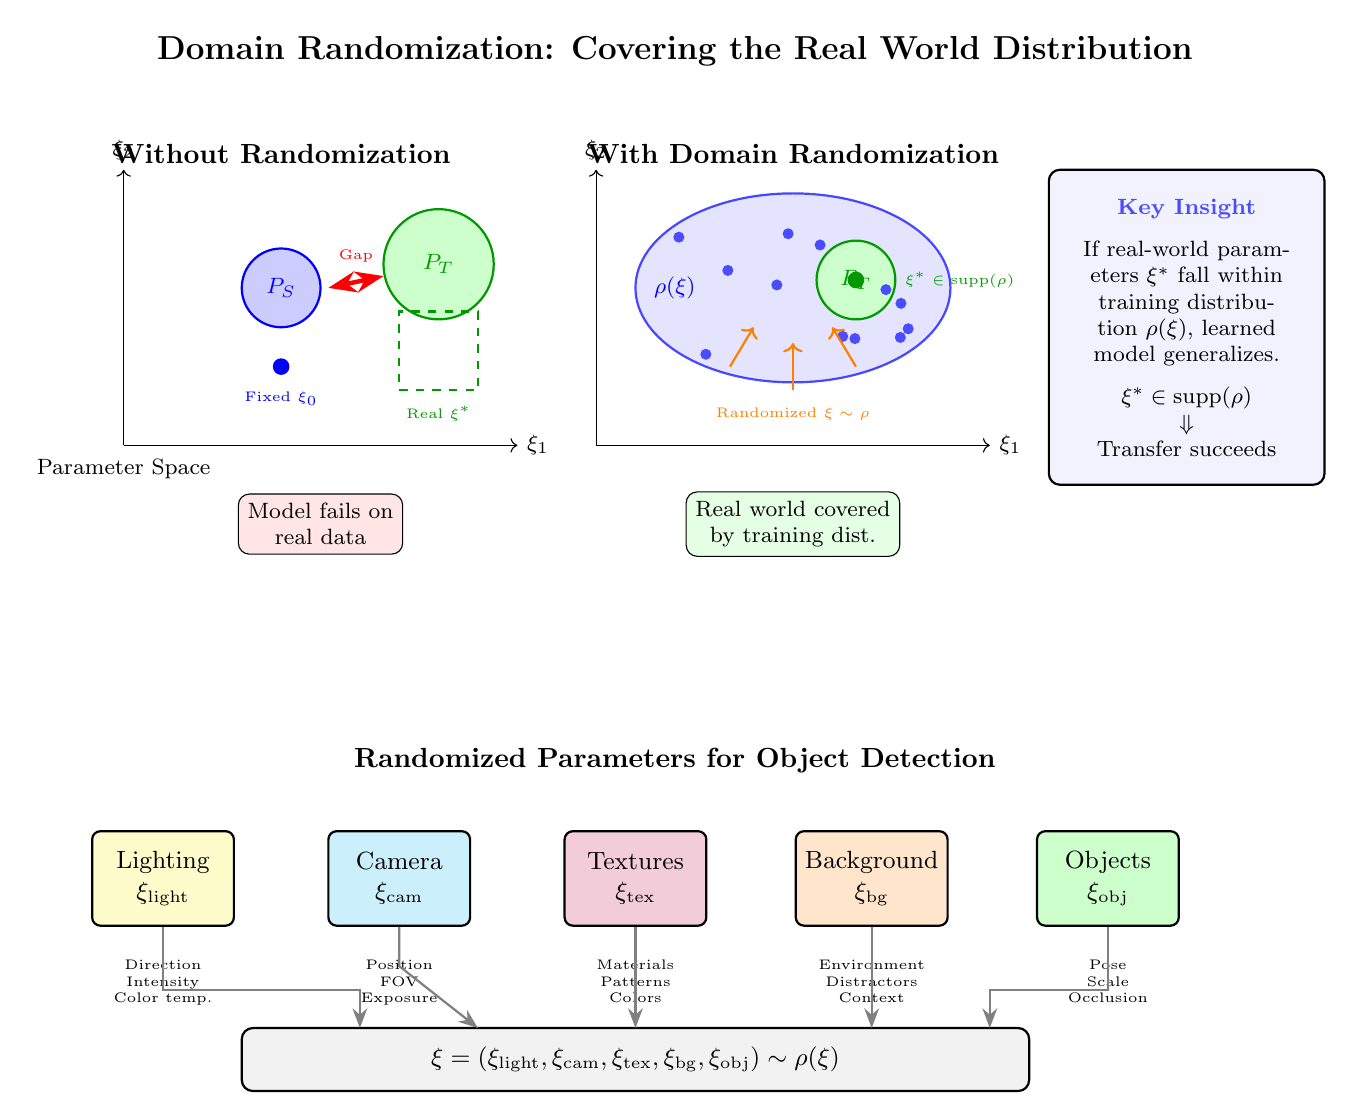
\begin{tikzpicture}[
    node distance=1cm,
    every node/.style={font=\small},
    box/.style={rectangle, draw, thick, minimum width=1.8cm, minimum height=1.2cm, align=center, rounded corners=3pt},
    arrow/.style={-{Stealth[length=2.5mm]}, thick},
    label/.style={font=\footnotesize}
]

% Title
\node[font=\bfseries\large] at (6.5, 5.5) {Domain Randomization: Covering the Real World Distribution};

% ============ LEFT: WITHOUT DOMAIN RANDOMIZATION ============
\begin{scope}[shift={(0, 0)}]
    \node[font=\bfseries] at (1.5, 4.2) {Without Randomization};

    % Single synthetic distribution (narrow)
    \draw[thick, blue, fill=blue!20] (1.5, 2.5) circle (0.5cm);
    \node[blue, font=\footnotesize] at (1.5, 2.5) {$P_S$};

    % Real world distribution (separate)
    \draw[thick, green!60!black, fill=green!20] (3.5, 2.8) circle (0.7cm);
    \node[green!60!black, font=\footnotesize] at (3.5, 2.8) {$P_T$};

    % Parameter space
    \draw[->] (-0.5, 0.5) -- (4.5, 0.5) node[right, font=\footnotesize] {$\xi_1$};
    \draw[->] (-0.5, 0.5) -- (-0.5, 4) node[above, font=\footnotesize] {$\xi_2$};
    \node[font=\footnotesize] at (-0.5, 0.2) {Parameter Space};

    % Single point for synthetic
    \fill[blue] (1.5, 1.5) circle (3pt);
    \node[blue, font=\tiny, below] at (1.5, 1.3) {Fixed $\xi_0$};

    % Real world region
    \draw[green!60!black, dashed, thick] (3, 1.2) -- (4, 1.2) -- (4, 2.2) -- (3, 2.2) -- cycle;
    \node[green!60!black, font=\tiny] at (3.5, 0.9) {Real $\xi^*$};

    % Gap indicator
    \draw[red, ultra thick, {Stealth}-{Stealth}] (2.1, 2.5) -- (2.8, 2.65);
    \node[red, font=\tiny, above] at (2.45, 2.7) {Gap};

    % Result annotation
    \node[draw, rounded corners, fill=red!10, font=\footnotesize, align=center] at (2, -0.5) {Model fails on\\real data};
\end{scope}

% ============ MIDDLE: STANDARD DOMAIN RANDOMIZATION ============
\begin{scope}[shift={(6, 0)}]
    \node[font=\bfseries] at (2, 4.2) {With Domain Randomization};

    % Large synthetic distribution covering real
    \draw[thick, blue, fill=blue!15, opacity=0.7] (2, 2.5) ellipse (2cm and 1.2cm);
    \node[blue, font=\footnotesize] at (0.5, 2.5) {$\rho(\xi)$};

    % Real world distribution (inside)
    \draw[thick, green!60!black, fill=green!20] (2.8, 2.6) circle (0.5cm);
    \node[green!60!black, font=\footnotesize] at (2.8, 2.6) {$P_T$};

    % Parameter space
    \draw[->] (-0.5, 0.5) -- (4.5, 0.5) node[right, font=\footnotesize] {$\xi_1$};
    \draw[->] (-0.5, 0.5) -- (-0.5, 4) node[above, font=\footnotesize] {$\xi_2$};

    % Multiple sampled points
    \foreach \i in {1,...,12} {
        \pgfmathsetmacro{\px}{2 + 1.6*rand}
        \pgfmathsetmacro{\py}{2.5 + 0.9*rand}
        \fill[blue!70] (\px, \py) circle (2pt);
    }

    % Real world point inside
    \fill[green!60!black] (2.8, 2.6) circle (3pt);
    \node[green!60!black, font=\tiny, right] at (3.3, 2.6) {$\xi^* \in \text{supp}(\rho)$};

    % Randomization arrows showing variation
    \draw[orange, thick, ->] (1.2, 1.5) -- (1.5, 2.0);
    \draw[orange, thick, ->] (2.8, 1.5) -- (2.5, 2.0);
    \draw[orange, thick, ->] (2, 1.2) -- (2, 1.8);
    \node[orange, font=\tiny] at (2, 0.9) {Randomized $\xi \sim \rho$};

    % Result annotation
    \node[draw, rounded corners, fill=green!10, font=\footnotesize, align=center] at (2, -0.5) {Real world covered\\by training dist.};
\end{scope}

% ============ BOTTOM: CONCEPT ILLUSTRATION ============
\begin{scope}[shift={(0, -5)}]
    \node[font=\bfseries] at (6.5, 1.5) {Randomized Parameters for Object Detection};

    % Lighting variations
    \begin{scope}[shift={(0, 0)}]
        \node[box, fill=yellow!20] (light) at (0, 0) {Lighting\\$\xi_{\text{light}}$};
        \node[font=\tiny, below=0.3cm of light, align=center] {Direction\\Intensity\\Color temp.};
    \end{scope}

    % Camera variations
    \begin{scope}[shift={(3, 0)}]
        \node[box, fill=cyan!20] (cam) at (0, 0) {Camera\\$\xi_{\text{cam}}$};
        \node[font=\tiny, below=0.3cm of cam, align=center] {Position\\FOV\\Exposure};
    \end{scope}

    % Texture variations
    \begin{scope}[shift={(6, 0)}]
        \node[box, fill=purple!20] (tex) at (0, 0) {Textures\\$\xi_{\text{tex}}$};
        \node[font=\tiny, below=0.3cm of tex, align=center] {Materials\\Patterns\\Colors};
    \end{scope}

    % Background variations
    \begin{scope}[shift={(9, 0)}]
        \node[box, fill=orange!20] (bg) at (0, 0) {Background\\$\xi_{\text{bg}}$};
        \node[font=\tiny, below=0.3cm of bg, align=center] {Environment\\Distractors\\Context};
    \end{scope}

    % Object variations
    \begin{scope}[shift={(12, 0)}]
        \node[box, fill=green!20] (obj) at (0, 0) {Objects\\$\xi_{\text{obj}}$};
        \node[font=\tiny, below=0.3cm of obj, align=center] {Pose\\Scale\\Occlusion};
    \end{scope}

    % Combined parameter vector
    \node[draw, thick, rounded corners, fill=gray!10, minimum width=10cm, minimum height=0.8cm] (combined) at (6, -2.3) {};
    \node at (6, -2.3) {$\xi = (\xi_{\text{light}}, \xi_{\text{cam}}, \xi_{\text{tex}}, \xi_{\text{bg}}, \xi_{\text{obj}}) \sim \rho(\xi)$};

    % Arrows to combined
    \draw[arrow, gray] (light.south) -- ++(0, -0.8) -| (2.5, -1.9);
    \draw[arrow, gray] (cam.south) -- ++(0, -0.5) -- (4, -1.9);
    \draw[arrow, gray] (tex.south) -- (6, -1.9);
    \draw[arrow, gray] (bg.south) -- ++(0, -0.5) -- (9, -1.9);
    \draw[arrow, gray] (obj.south) -- ++(0, -0.8) -| (10.5, -1.9);
\end{scope}

% ============ RIGHT SIDE: KEY INSIGHT ============
\begin{scope}[shift={(13, 2)}]
    \node[draw, thick, rounded corners, fill=blue!5, minimum width=3.5cm, minimum height=4cm, align=center] (insight) at (0, 0) {};
    \node[font=\bfseries\footnotesize, blue!70] at (0, 1.5) {Key Insight};
    \node[font=\footnotesize, align=center, text width=3cm] at (0, 0.3) {
        If real-world parameters $\xi^*$ fall within training distribution $\rho(\xi)$, learned model generalizes.
    };
    \node[font=\footnotesize, align=center] at (0, -1.2) {$\xi^* \in \text{supp}(\rho)$\\$\Downarrow$\\Transfer succeeds};
\end{scope}

\end{tikzpicture}
\end{document}
